\chapter{Analysis of Collected Data}
\label{chap:analysis}

\begin{itemize}
\item Analyses of data collected in 4 months (between 2017-11-10 and 2018-03-09).
\item Goals: validate that the system works, get insight into how it works
  and what can/should be improved.
\end{itemize}


\section{Data Description}

\begin{itemize}
\item About 1000 users who tackled at least one task (but not necessarily solved
  it), 800 students who solved at least one task. Caveat: A single user may be
  counted multiple times if he didn't sign up and the session cookie expired.)
\item 100 returning students (= student who solved a task session in at
  least two distinct days)
  (complete engagement curves in figure \ref{fig:engagement-curves}).
\item 11K task sessions (with at least one edit), 960 of them solved
  (resulting in the overall success rate $86 \%$).
\item Solving time median is 60s (interquartile range: 24-145s) - lognormal
  distribution - REF to figure; so the mean is much higher (even the time is
  capped at 1h): 195s, with high standard deviation of 496s.
\item Program snapshots: 180K, taken at edits (140K), and executions (40K).
\end{itemize}

% TODO (GA):
% Desktop 94%, Mobile 4%, Tablet 2%

%\section{Metrics}

% TODO: join with another plot (-> two plots on a single line).
\imgW{daily-task-sessions}{%
  Daily number of solved task sessions (weekly average).}

\begin{figure}[htb]
\begin{center}
  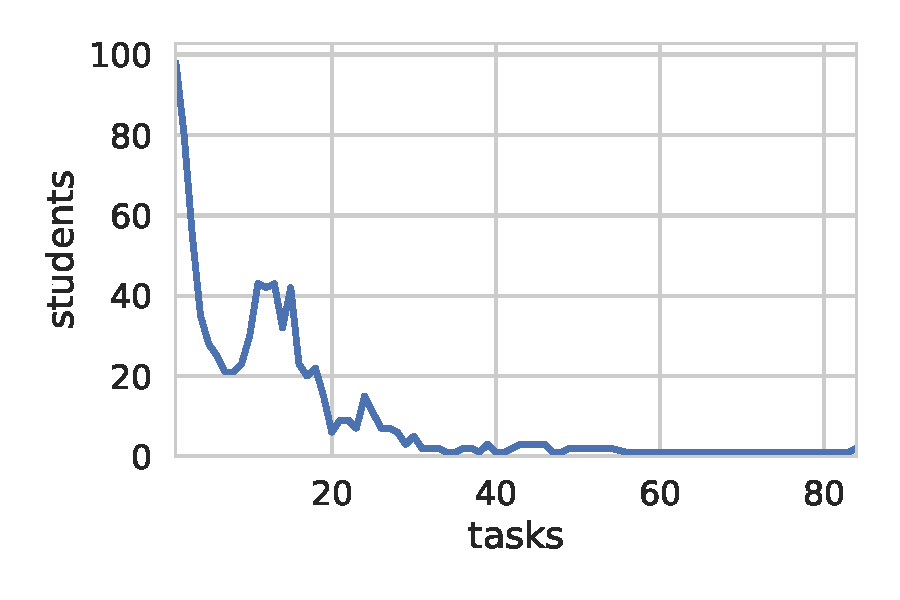
\includegraphics[width=0.48\textwidth]{img/engagement-tasks}
  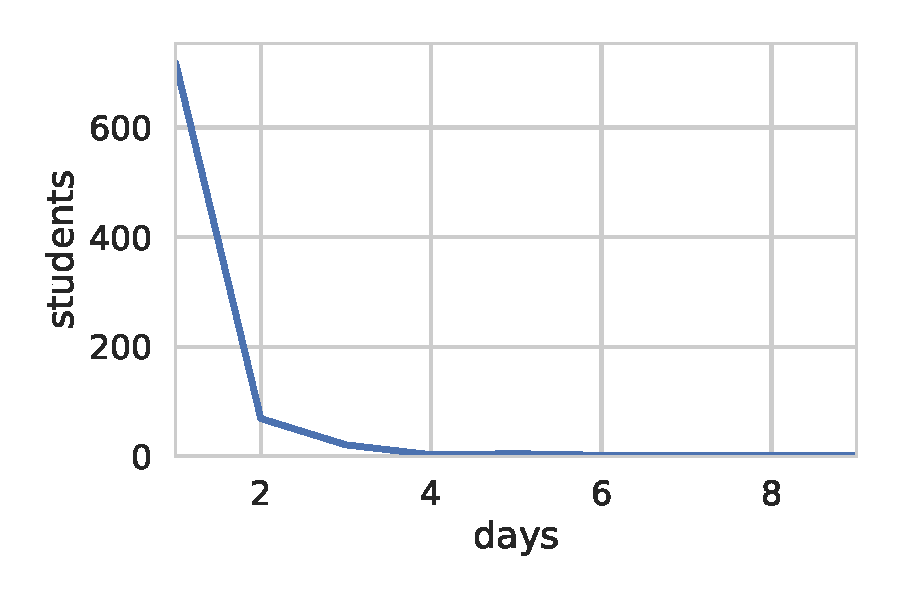
\includegraphics[width=0.48\textwidth]{img/engagement-days}
\end{center}
\caption{%
  Engagement curves.
  Left: How many students solved given number of tasks.
  Right: How many students solved a task given number of days.}
\label{fig:engagement-curves}
\end{figure}

\begin{figure}[htb]
\begin{center}
  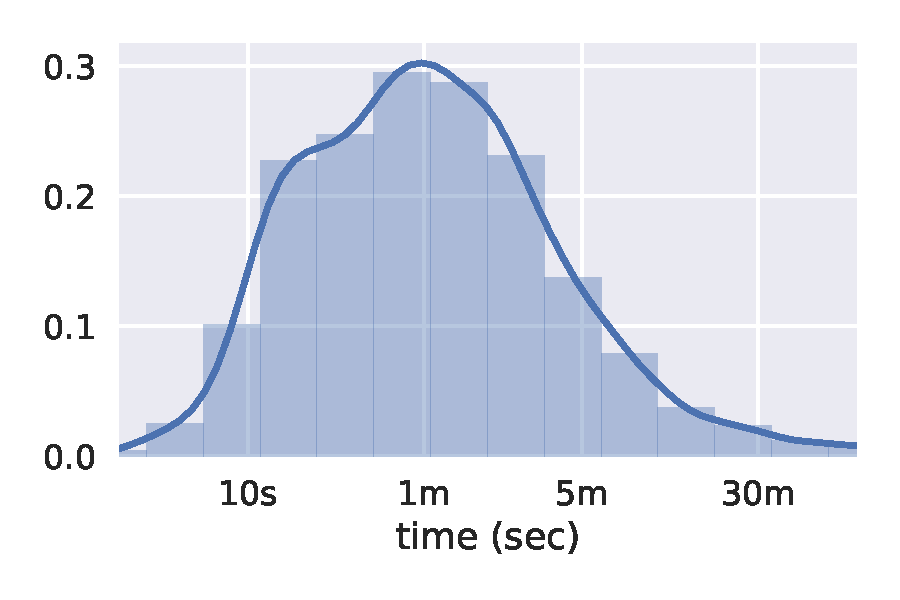
\includegraphics[width=0.48\textwidth]{img/task-sessions-time-log}
  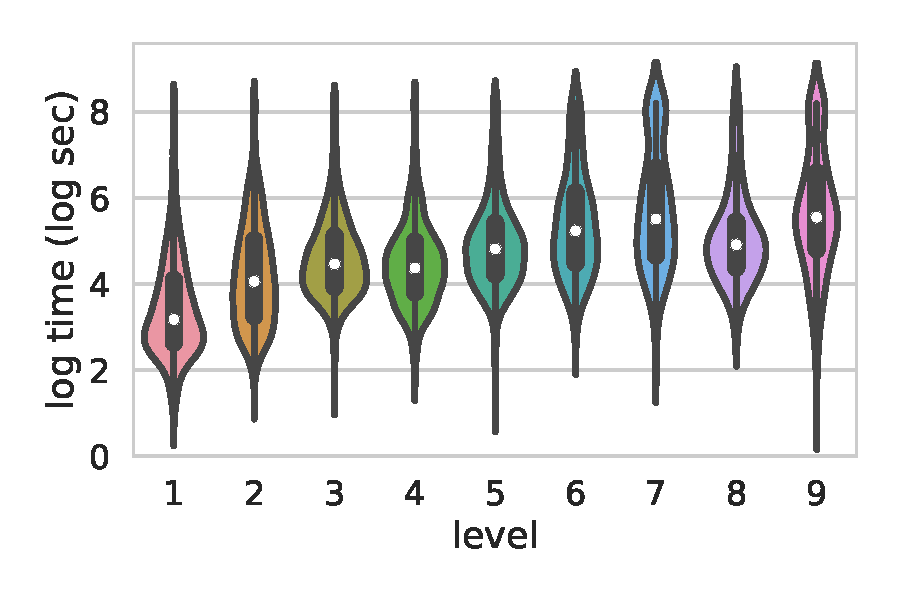
\includegraphics[width=0.48\textwidth]{img/levels-time}
\end{center}
\caption{%
  Distribution of log-transformed solving times.
  Left: All task sessions.
  Right: For each level.}
\label{fig:solving-times}
\end{figure}


\section{Task Difficulties}

\begin{itemize}
\item Q: Are tasks in levels homogenuous (wrt. their difficulty)?
\item Q: Is difficulty increasing with higher levels?
\end{itemize}

\imgW{difficulties-tasks-levels}{%
  Difficulties (spent times and number of edits, both log-transformed)
  of tasks in each level.}


\section{Performance Analysis}

\begin{itemize}
\item What is a reasonable performance compression?
  (REF to the discussion in prev. chapters - possibilities and what is used in
  our system)
\item Overall correlation between time spent and number of edits (both log-transformed)
  is quite high (0.73).
\item Within tasks: median correlation 0.64, interquartile range 0.5 -- 0.72.
  Distribution: figure \ref{fig:time-vs-edits}.
\end{itemize}

\begin{figure}[htb]
\begin{center}
  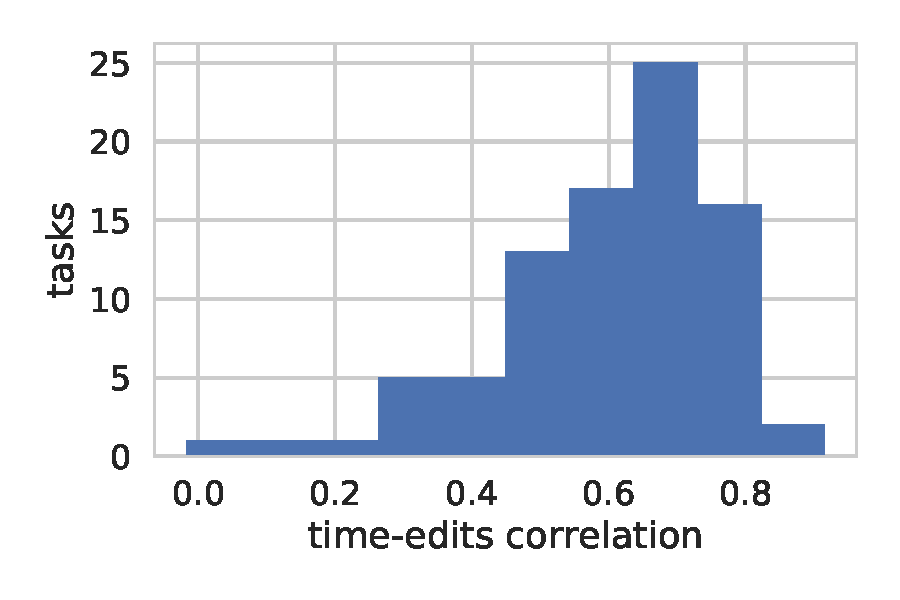
\includegraphics[width=0.48\textwidth]{img/time-edits-corr}
  %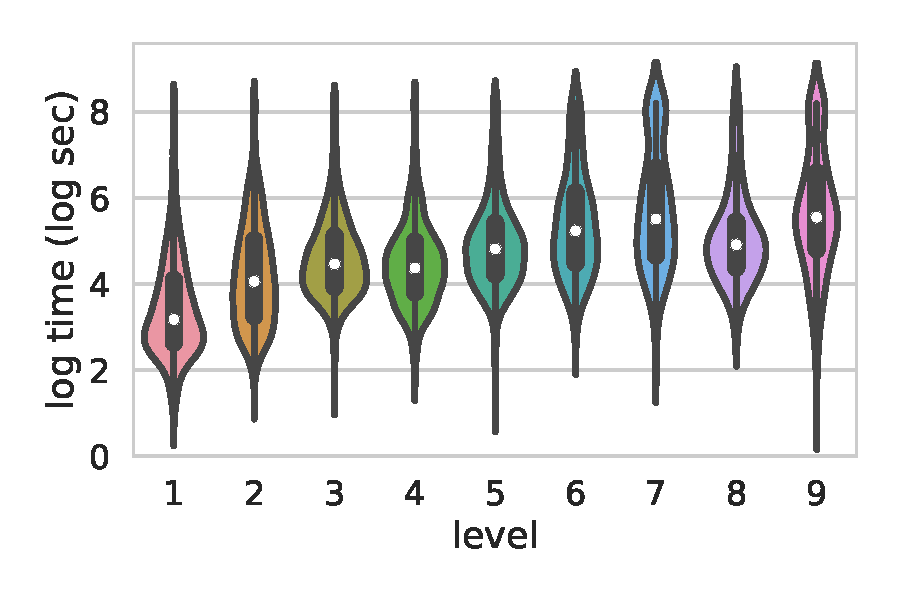
\includegraphics[width=0.48\textwidth]{img/levels-time}
\end{center}
\caption{%
  Distribution of Pearson correlations between solving times and number of edits
  (both log-transformed). TODO: another plot on the right.}
\label{fig:time-vs-edits}
\end{figure}
